\chapter{Bilder}
\label{anhang:chapter-bilder}

\section{Spielverläufe}
\label{anhang:section-bilder-spielverlaeufe}

\vspace*{-0.25cm}

% Alternative 1
% walk 2
% take 12
% take 32
% walk 2
% take 17
% take 10
% take 30
% take 4
% take 1
% take 26
% take 3
% take 20
% walk 2
% take 11
% parallel
%     take 6, walk 1, take 22
%     take 6, take 22, walk 1
%     take 22, walk 1, take 6
%     take 22, take 6, walk 1
% walk 1
% take 16
\begin{figure}[!ht]
    \centering
    \begin{adjustbox}{width=\textwidth,keepaspectratio}
        \begin{tikzpicture}[
                arrow/.style={->, very thick, shorten >=2pt, shorten <=2pt}
            ]

            \tikzset{
                take/.style={inner sep=0,outer sep=0, label=below:#1 nehmen},
            }

            % start
            \node[draw, circle, inner sep=2pt, label=below:Start] (start) at (0,0) {};

            % walk 2
            \node[right = of start] (walk2a) {2 laufen};
            \draw[arrow] (start) -- (walk2a);

            % take 12
            \node[take=12, right = of walk2a] (take12) {\includegraphics[width=15mm]{res/pictures/assets/12-front.png}};
            \draw[arrow] (walk2a) -- (take12);

            % take 32
            \node[take=32, right = of take12] (take32) {\includegraphics[width=20mm]{res/pictures/assets/32-front.png}};
            \draw[arrow] (take12) -- (take32);

            % walk 2
            \node[right = of take32] (walk2b) {2 laufen};
            \draw[arrow] (take32) -- (walk2b);

            % take 17
            \node[take=17, right = of walk2b] (take17) {\includegraphics[width=15mm]{res/pictures/assets/17-front.png}};
            \draw[arrow] (walk2b) -- (take17);

            % take 10
            \node[take=10, right = of take17] (take10) {\includegraphics[width=10mm]{res/pictures/assets/10-front.png}};
            \draw[arrow] (take17) -- (take10);

            % take 30
            \node[take=30, right = of take10] (take30) {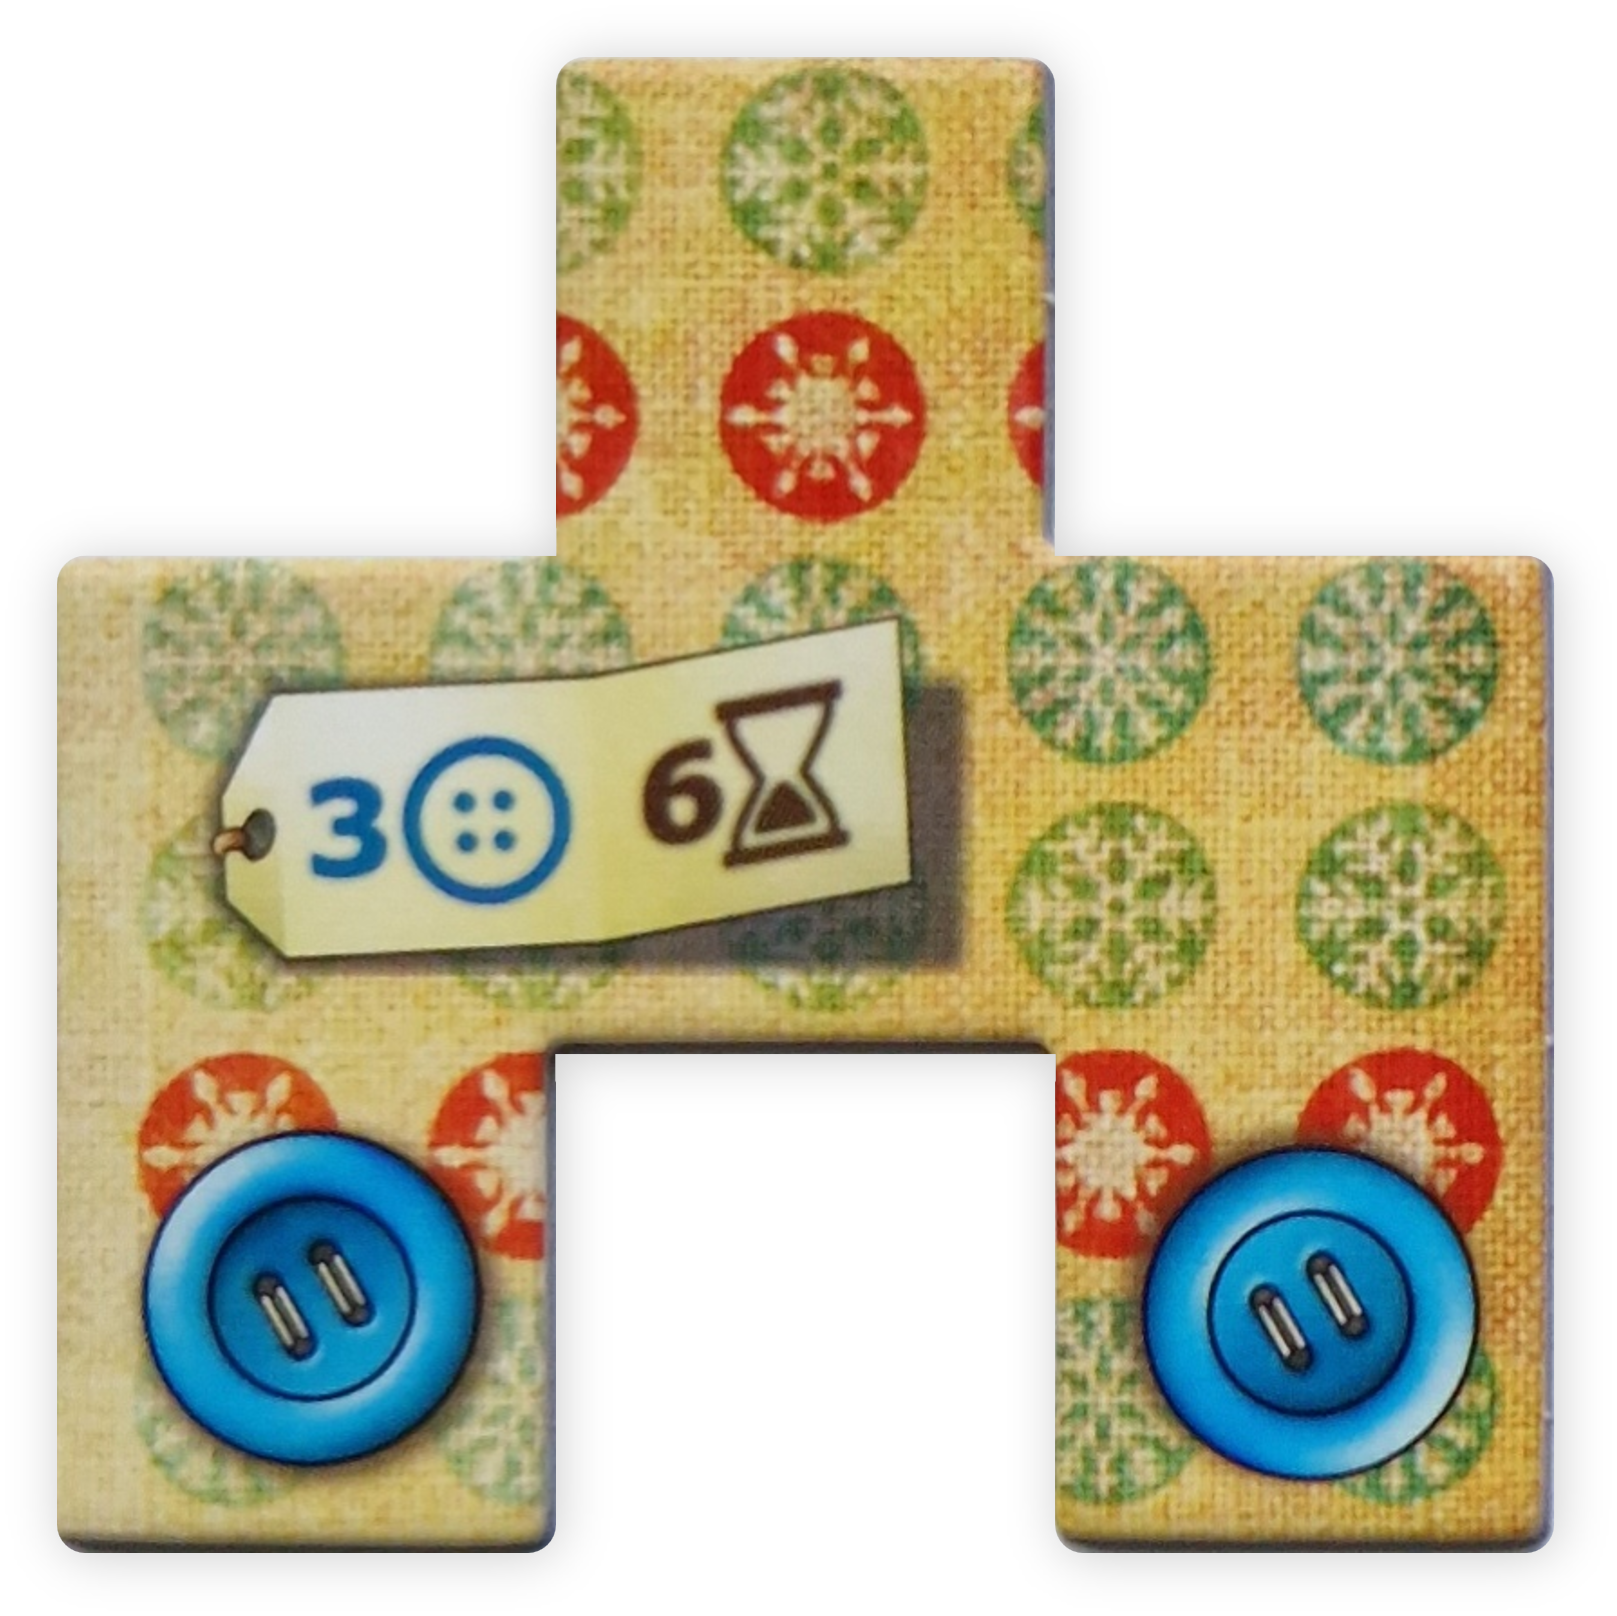
\includegraphics[width=15mm]{res/pictures/assets/30-front.png}};
            \draw[arrow] (take10) -- (take30);

            % take 4
            \node[take=4, right = of take30] (take04) {\includegraphics[width=15mm]{res/pictures/assets/04-front.png}};
            \draw[arrow] (take30) -- (take04);

            % take 1
            \node[take=1, right = of take04] (take01) {\includegraphics[width=15mm]{res/pictures/assets/01-front.png}};
            \draw[arrow] (take04) -- (take01);

            % take 26
            \node[take=26, right = of take01] (take26) {\includegraphics[width=10mm]{res/pictures/assets/26-front.png}};
            \draw[arrow] (take01) -- (take26);

            % take 3  (down)
            \node[take=3, below = 1.95cm of take26] (take03) {\includegraphics[width=15mm]{res/pictures/assets/03-front.png}};
            \draw[arrow, shorten <=20pt] (take26) -- (take03);

            % take 20 (down)
            \node[take=20, below = 1.95cm of take03] (take20) {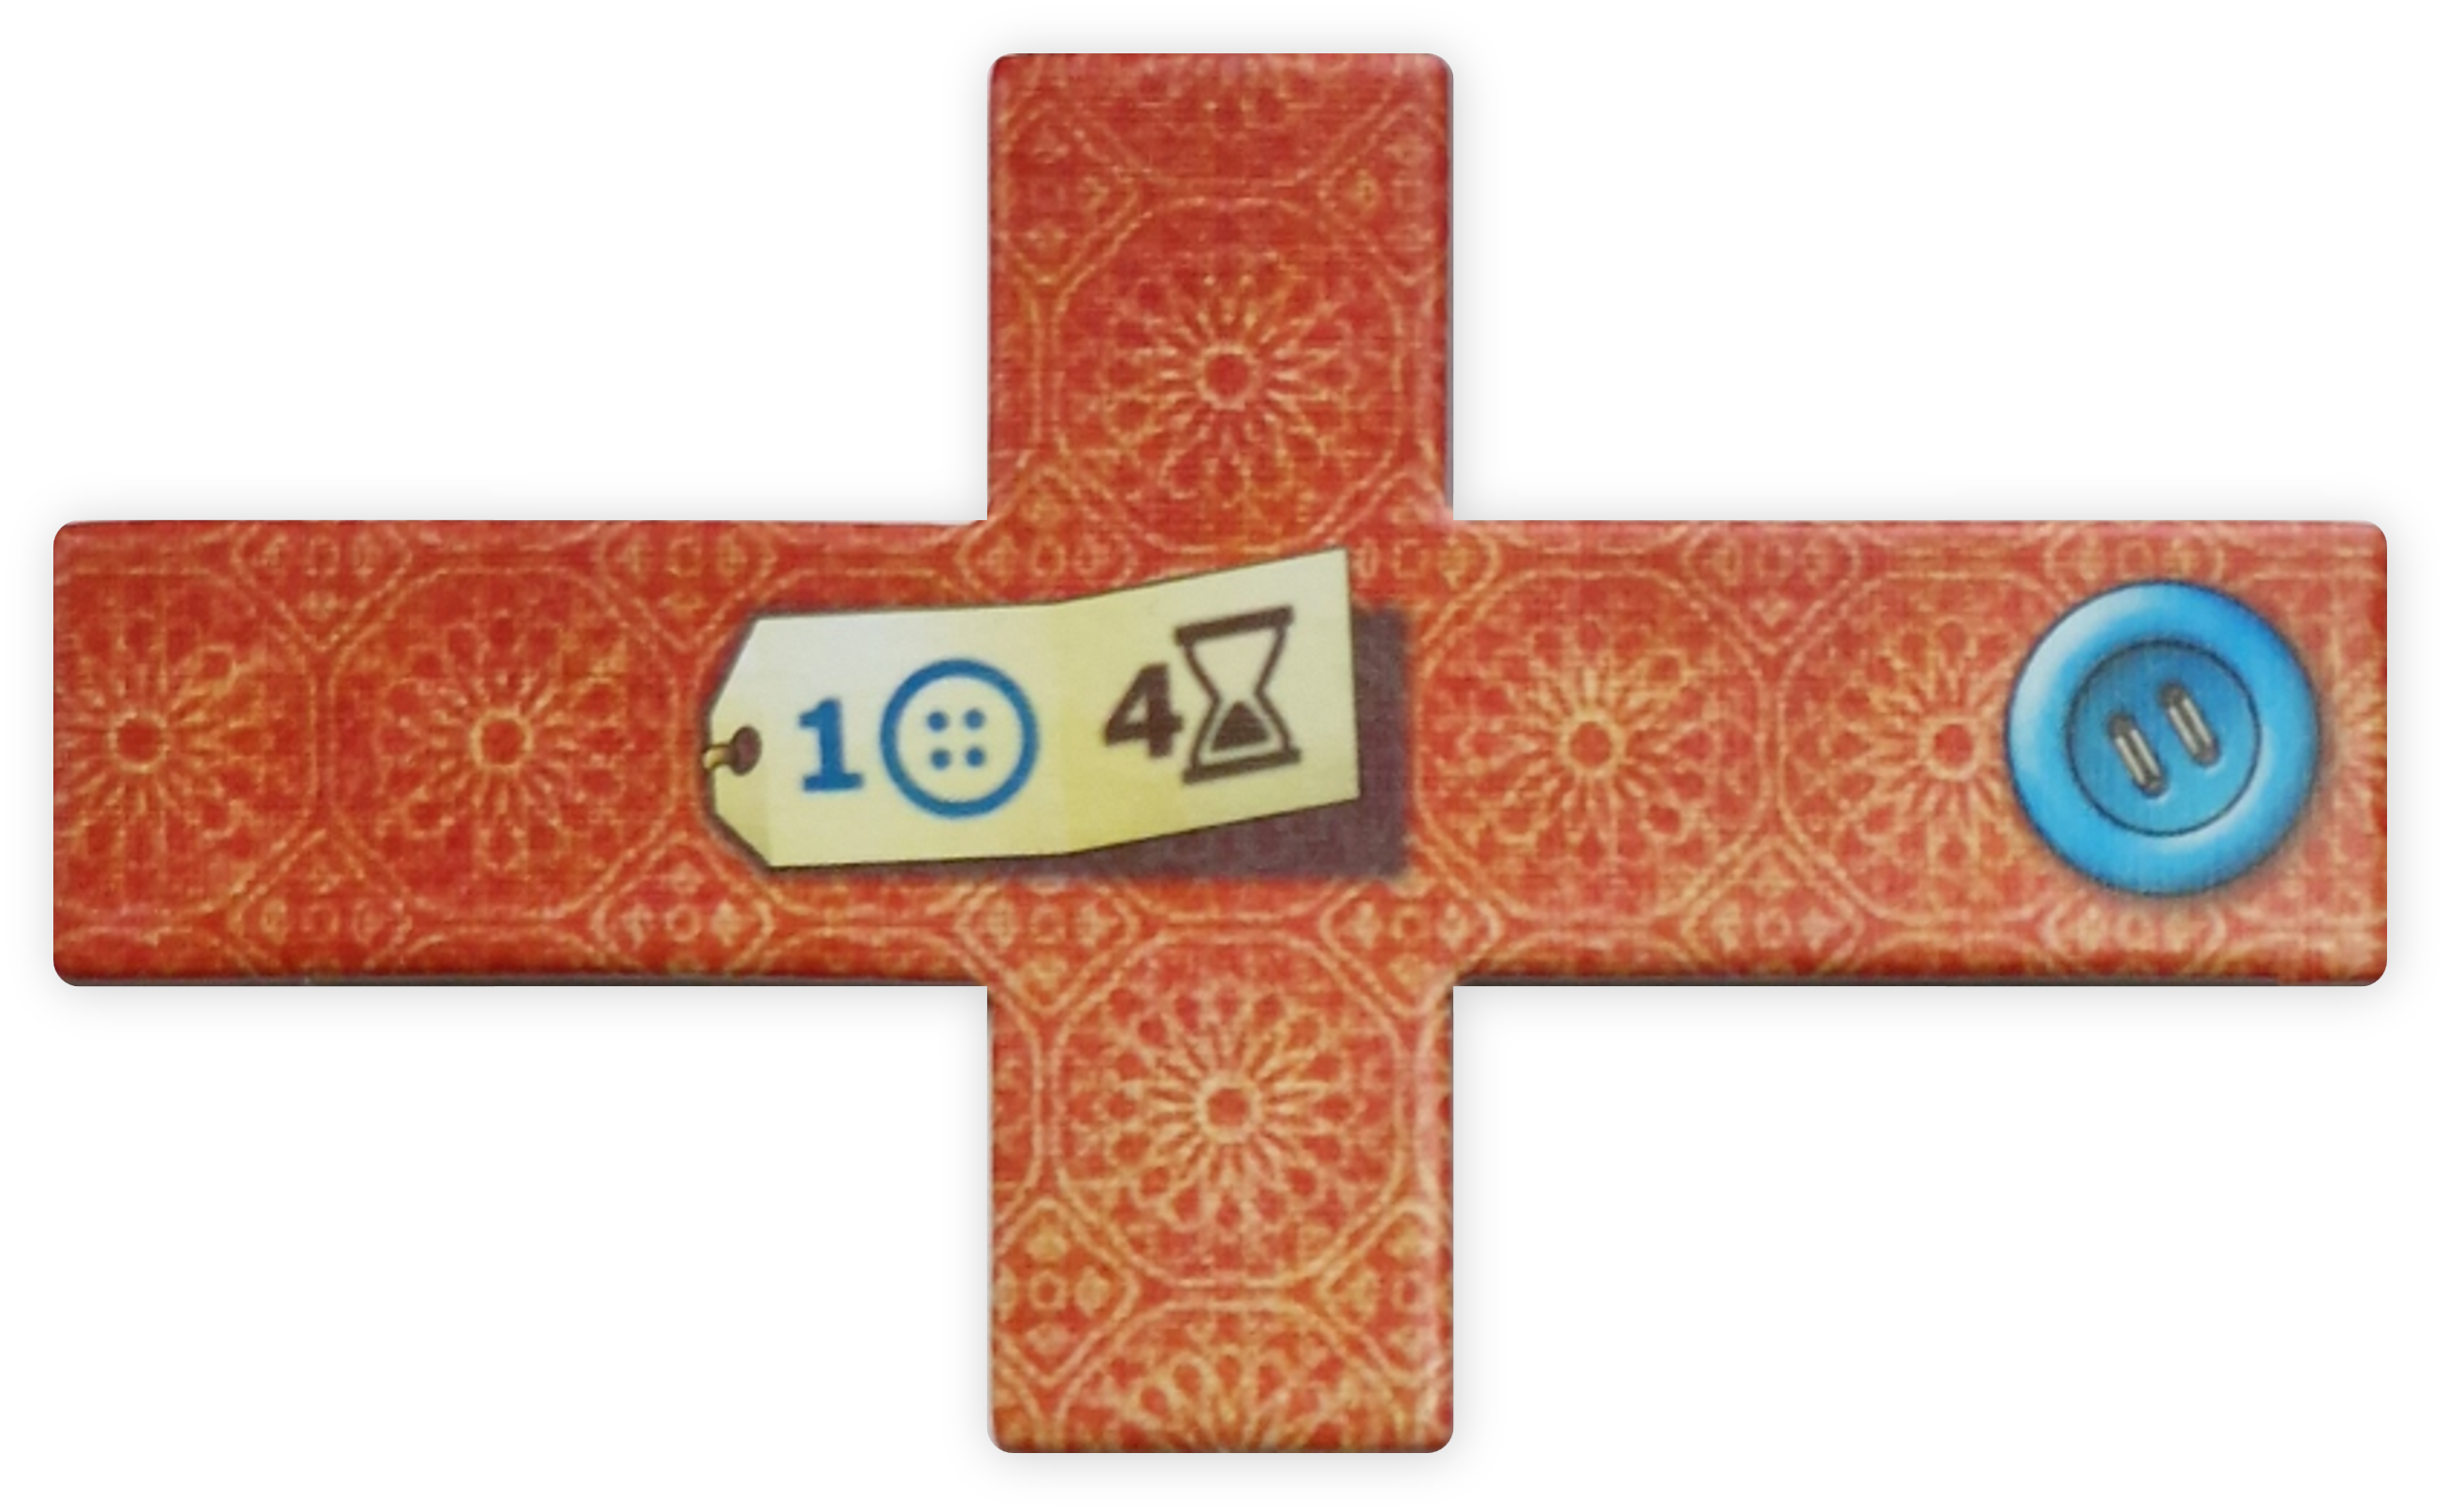
\includegraphics[width=25mm]{res/pictures/assets/20-front.png}};
            \draw[arrow, shorten <=20pt] (take03) -- (take20);

            % walk 2
            \node[left = of take20] (walk2c) {2 laufen};
            \draw[arrow] (take20) -- (walk2c);

            % take 11
            \node[take=11, left = of walk2c] (take11) {\includegraphics[width=20mm]{res/pictures/assets/11-front.png}};
            \draw[arrow] (walk2c) -- (take11);

            % parallel
            %     b) take 6, take 22, walk 1
            \node[take=6, above left = -0.215cm and 2.5cm of take11] (take06b) {\includegraphics[width=15mm]{res/pictures/assets/06-front.png}};
            \node[take=22, left = of take06b] (take22b) {\includegraphics[width=15mm]{res/pictures/assets/22-front.png}};
            \node[left = of take22b] (walk1b) {1 laufen};
            \draw[arrow] (take11) -|-[ratio=.5] (take06b);
            \draw[arrow] (take06b) -- (take22b);
            \draw[arrow] (take22b) -- (walk1b);

            %     a) take 6, walk 1, take 22
            \node[take=6, above = 0.8cm of take06b] (take06a) {\includegraphics[width=15mm]{res/pictures/assets/06-front.png}};
            \node[left = of take06a] (walk1a) {1 laufen};
            \node[take=22, left = of walk1a] (take22a) {\includegraphics[width=15mm]{res/pictures/assets/22-front.png}};
            \draw[arrow] (take11) -|-[ratio=.5] (take06a);
            \draw[arrow] (take06a) -- (walk1a);
            \draw[arrow] (walk1a) -- (take22a);

            %     c) take 22, walk 1, take 6
            \node[take=22, below left = -0.215cm and 2.5cm of take11] (take22c) {\includegraphics[width=15mm]{res/pictures/assets/22-front.png}};
            \node[left = of take22c] (walk1c) {1 laufen};
            \node[take=6, left = of walk1c] (take06c) {\includegraphics[width=15mm]{res/pictures/assets/06-front.png}};
            \draw[arrow] (take11) -|-[ratio=.5] (take22c);
            \draw[arrow] (take22c) -- (walk1c);
            \draw[arrow] (walk1c) -- (take06c);

            %     d) take 22, take 6, walk 1
            \node[take=22, below=1.25cm of take22c] (take22d) {\includegraphics[width=15mm]{res/pictures/assets/22-front.png}};
            \node[take=6, left = of take22d] (take06d) {\includegraphics[width=15mm]{res/pictures/assets/06-front.png}};
            \node[left = of take06d] (walk1d) {1 laufen};
            \draw[arrow] (take11) -|-[ratio=.5] (take22d);
            \draw[arrow] (take22d) -- (take06d);
            \draw[arrow] (take06d) -- (walk1d);

            % walk 1
            \node[left = 3.5cm of take11 -| walk1d] (walk1e) {2 laufen};
            \draw[arrow] (walk1b) -|-[ratio=.5] (walk1e);
            \draw[arrow] (take22a) -|-[ratio=.5] (walk1e);
            \draw[arrow] (take06c) -|-[ratio=.5] (walk1e);
            \draw[arrow] (walk1d) -|-[ratio=.5] (walk1e);

            % take 16
            \node[take=16, left = of walk1e] (take16) {\includegraphics[width=10mm]{res/pictures/assets/16-front.png}};
            \draw[arrow] (walk1e) -- (take16);

            % end
            \node[draw, circle, inner sep=2pt, label=below:Ende] (end) at (start |- take16)  {};
            \draw[arrow] (take16) -- (end);
        \end{tikzpicture}
    \end{adjustbox}
    \vspace*{-0.7cm}
    \caption{Perfektes Patchwork Spiel \textendash{} Alternative 1}
    \label{fig:max-score-turns-alternative-1}
\end{figure}

\vspace*{-0.3cm}

% Alternative 2
% walk 2
% take 12
% take 32
% walk 2
% take 17
% take 10
% take 30
% take 3
% take 1
% take 26
% take 2
% walk 1
% walk 2
% take 20
% parallel
%     walk 4, take 6, take 11, walk 1
%     walk 4, take 6, walk 1, take 11
%     walk 4, take 11, walk 1, take 4
%     walk 4, take 11, take 4, walk 1
%     take 6, walk 5, take 11
%     take 11, walk 5, take 6
%     take 6, take 11, walk 3, walk 2
%     take 11, take 6, walk 3, walk 2
% take 16
\begin{figure}[!ht]
    \centering
    \begin{adjustbox}{width=\textwidth,keepaspectratio}
        \begin{tikzpicture}[
                arrow/.style={->, very thick, shorten >=2pt, shorten <=2pt}
            ]

            \tikzset{
                take/.style={inner sep=0,outer sep=0, label=below:#1 nehmen},
            }

            % start
            \node[draw, circle, inner sep=2pt, label=below:Start] (start) at (0,0) {};

            % walk 2
            \node[right = of start] (walk2a) {2 laufen};
            \draw[arrow] (start) -- (walk2a);

            % take 12
            \node[take=12, right = of walk2a] (take12) {\includegraphics[width=15mm]{res/pictures/assets/12-front.png}};
            \draw[arrow] (walk2a) -- (take12);

            % take 32
            \node[take=32, right = of take12] (take32) {\includegraphics[width=20mm]{res/pictures/assets/32-front.png}};
            \draw[arrow] (take12) -- (take32);

            % walk 2
            \node[right = of take32] (walk2b) {2 laufen};
            \draw[arrow] (take32) -- (walk2b);

            % take 17
            \node[take=17, right = of walk2b] (take17) {\includegraphics[width=15mm]{res/pictures/assets/17-front.png}};
            \draw[arrow] (walk2b) -- (take17);

            % take 10
            \node[take=10, right = of take17] (take10) {\includegraphics[width=10mm]{res/pictures/assets/10-front.png}};
            \draw[arrow] (take17) -- (take10);

            % take 30
            \node[take=30, right = of take10] (take30) {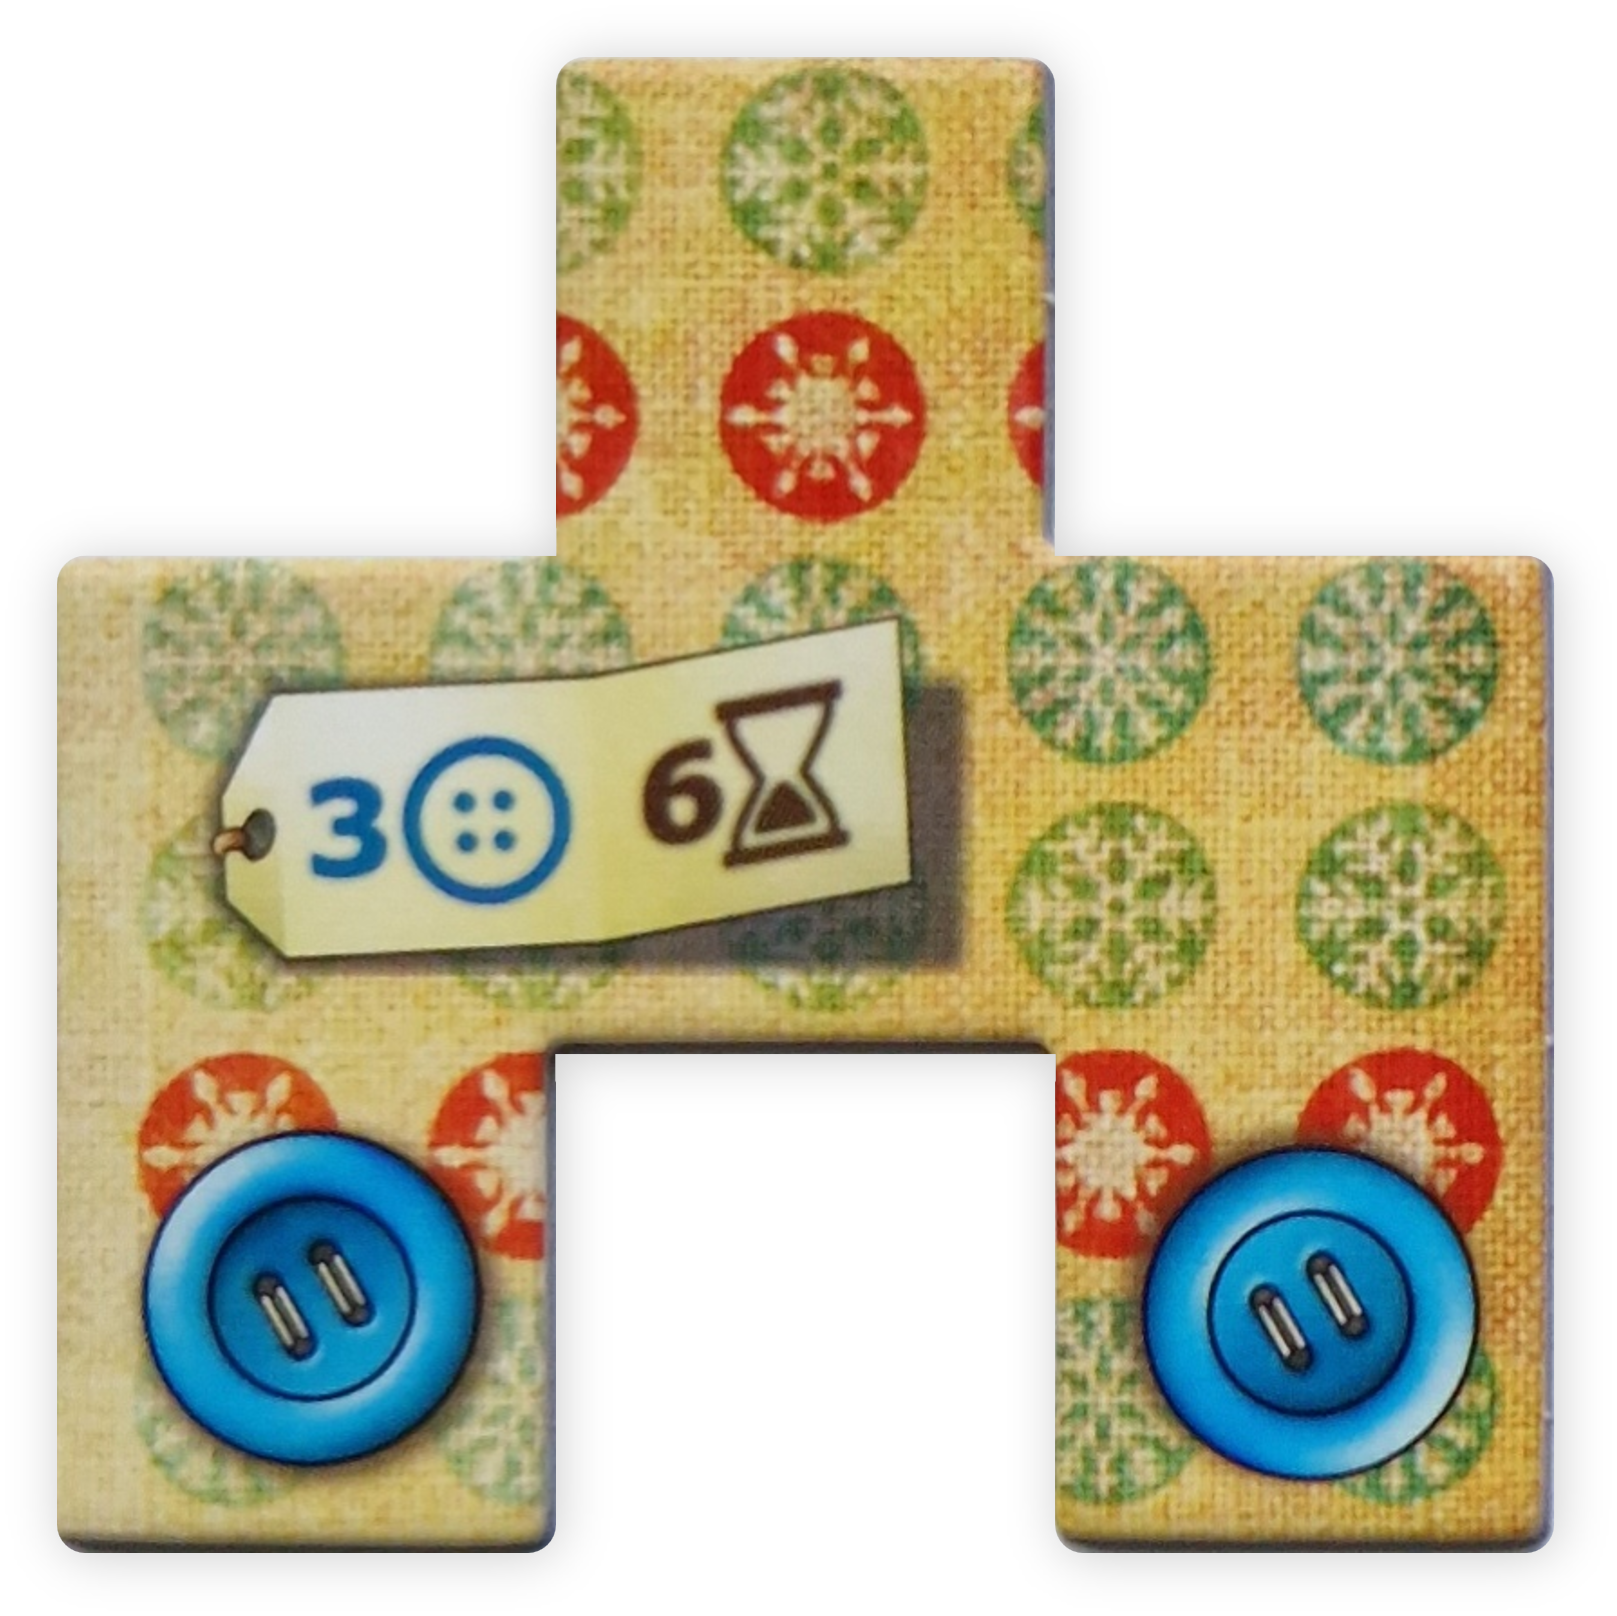
\includegraphics[width=15mm]{res/pictures/assets/30-front.png}};
            \draw[arrow] (take10) -- (take30);

            % take 3
            \node[take=3, right = of take30] (take03) {\includegraphics[width=15mm]{res/pictures/assets/03-front.png}};
            \draw[arrow] (take30) -- (take03);

            % take 1
            \node[take=1, right = of take03] (take01) {\includegraphics[width=15mm]{res/pictures/assets/01-front.png}};
            \draw[arrow] (take03) -- (take01);

            % take 26
            \node[take=26, right = of take01] (take26) {\includegraphics[width=10mm]{res/pictures/assets/26-front.png}};
            \draw[arrow] (take01) -- (take26);

            % take 2 (down)
            \node[take=2, below = 2.65cm of take26] (take02) {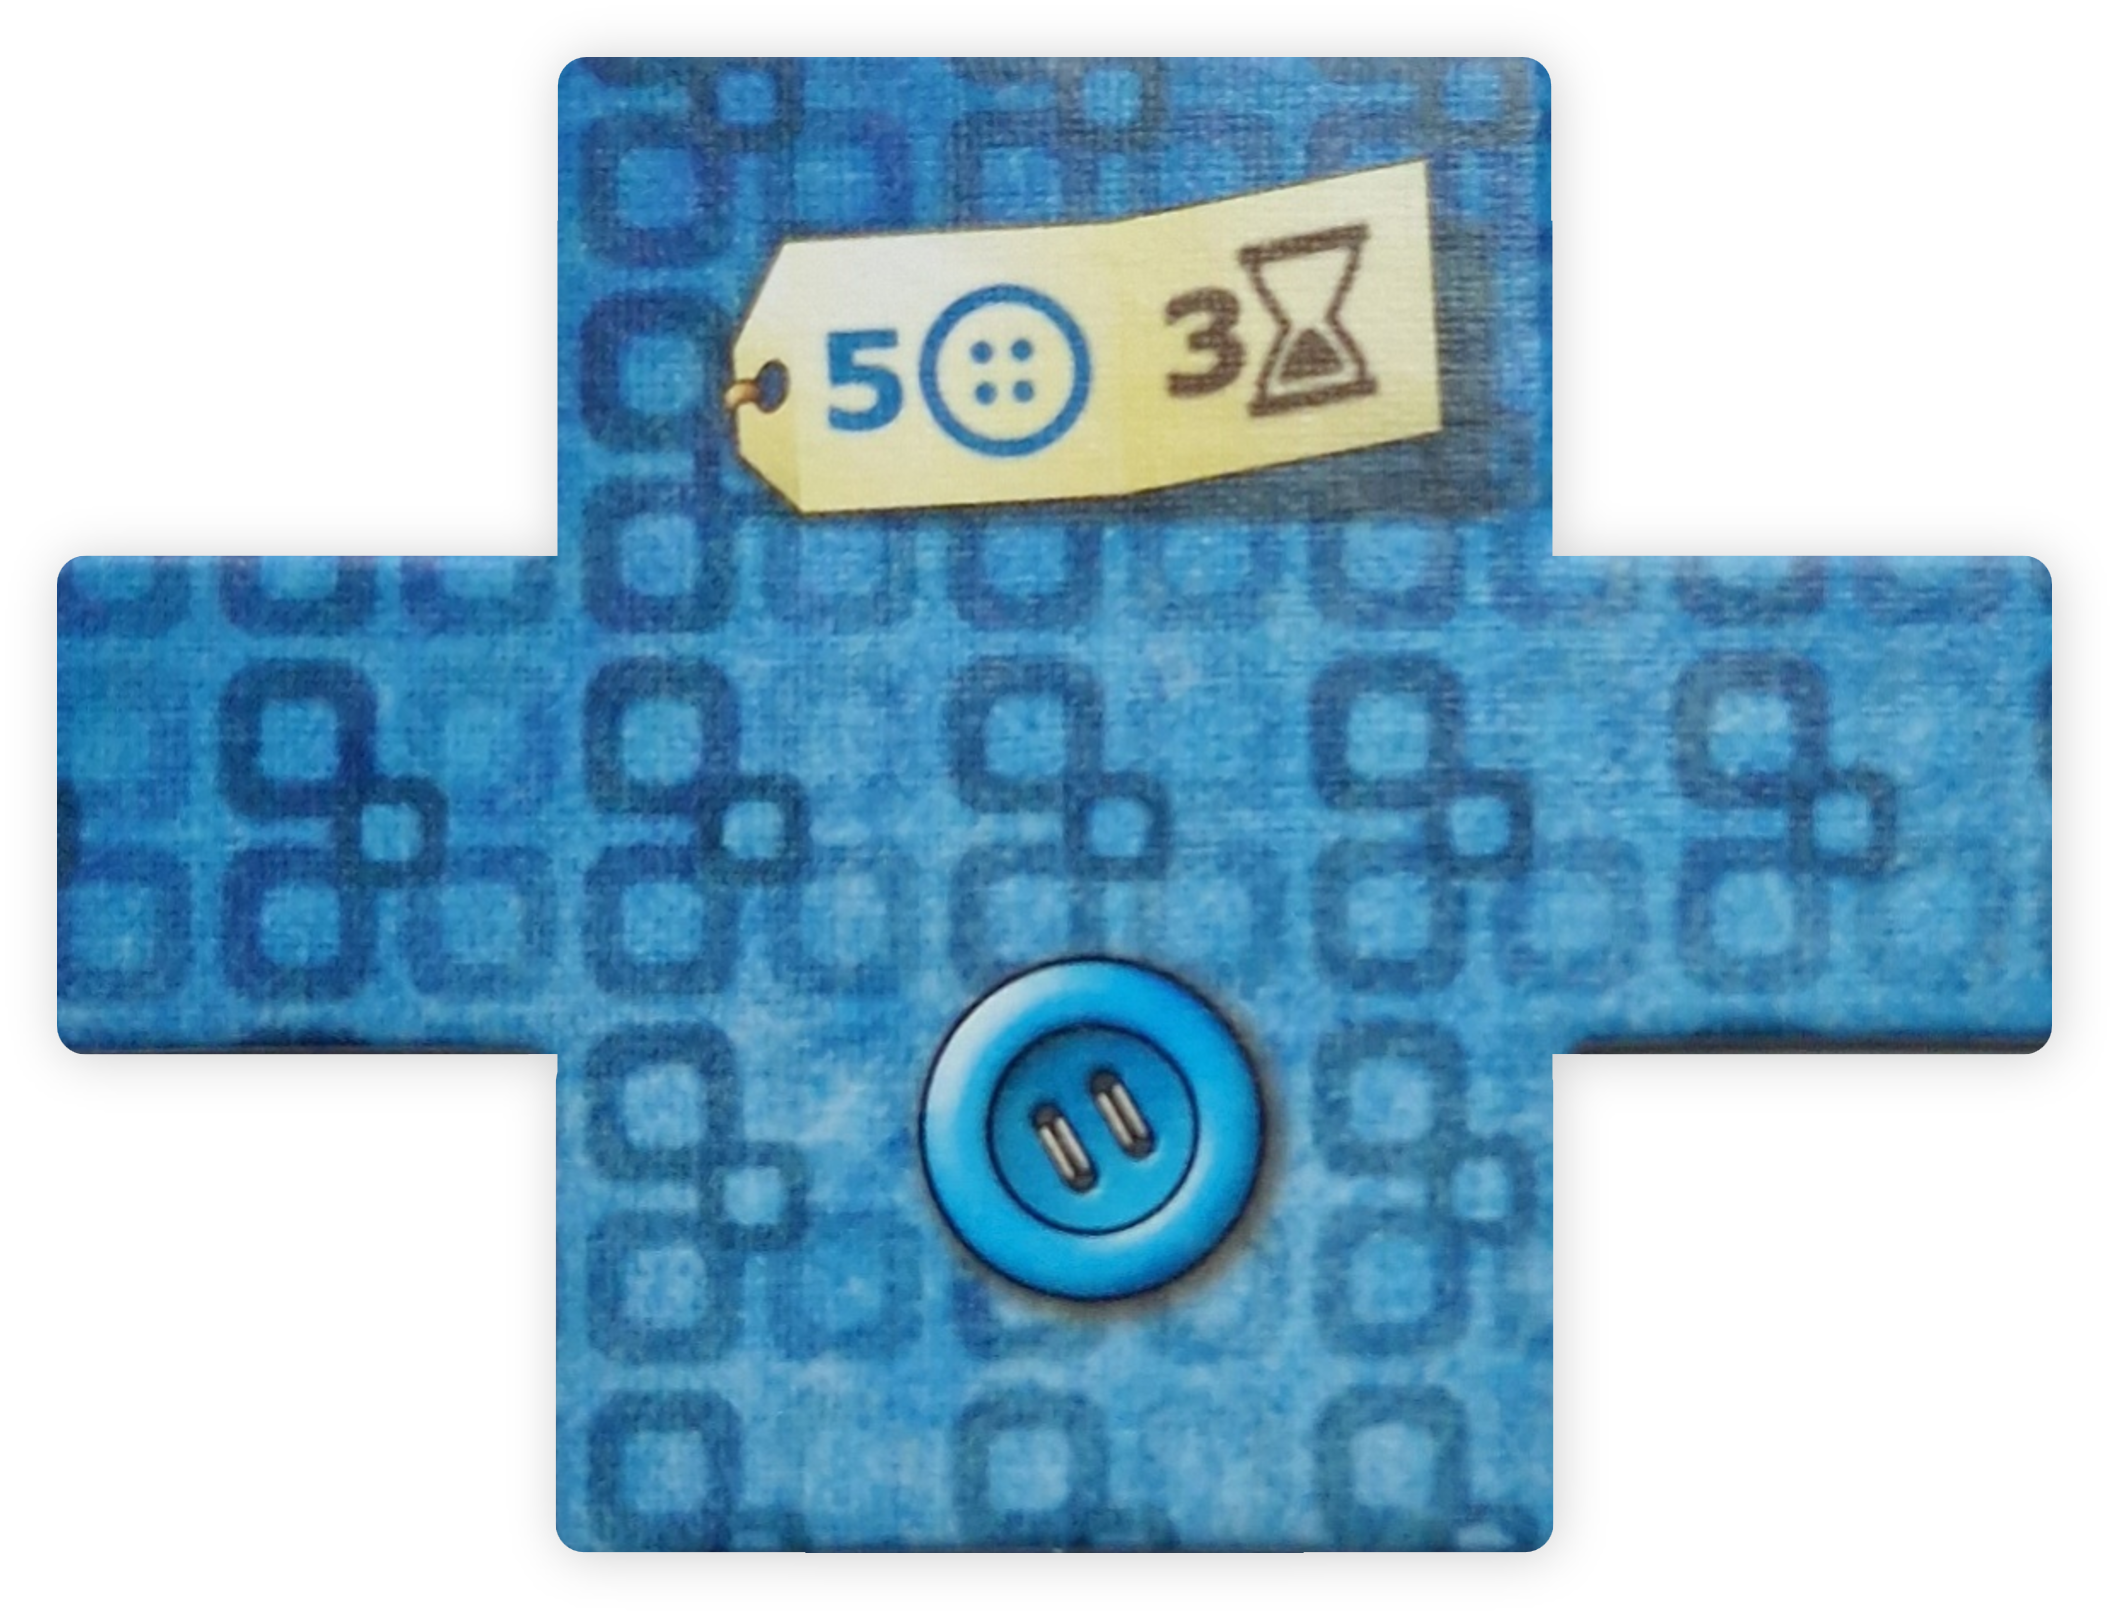
\includegraphics[width=20mm]{res/pictures/assets/02-front.png}};
            \draw[arrow, shorten <=20pt] (take26) -- (take02);

            % walk 1 (down)
            \node[, below = 2.65cm of take02] (walk1a) {1 laufen};
            \draw[arrow, shorten <=20pt] (take02) -- (walk1a);

            % walk 2
            \node[left = of walk1a] (walk2c) {2 laufen};
            \draw[arrow] (walk1a) -- (walk2c);

            % take 20
            \node[take=20, left = of walk2c] (take20) {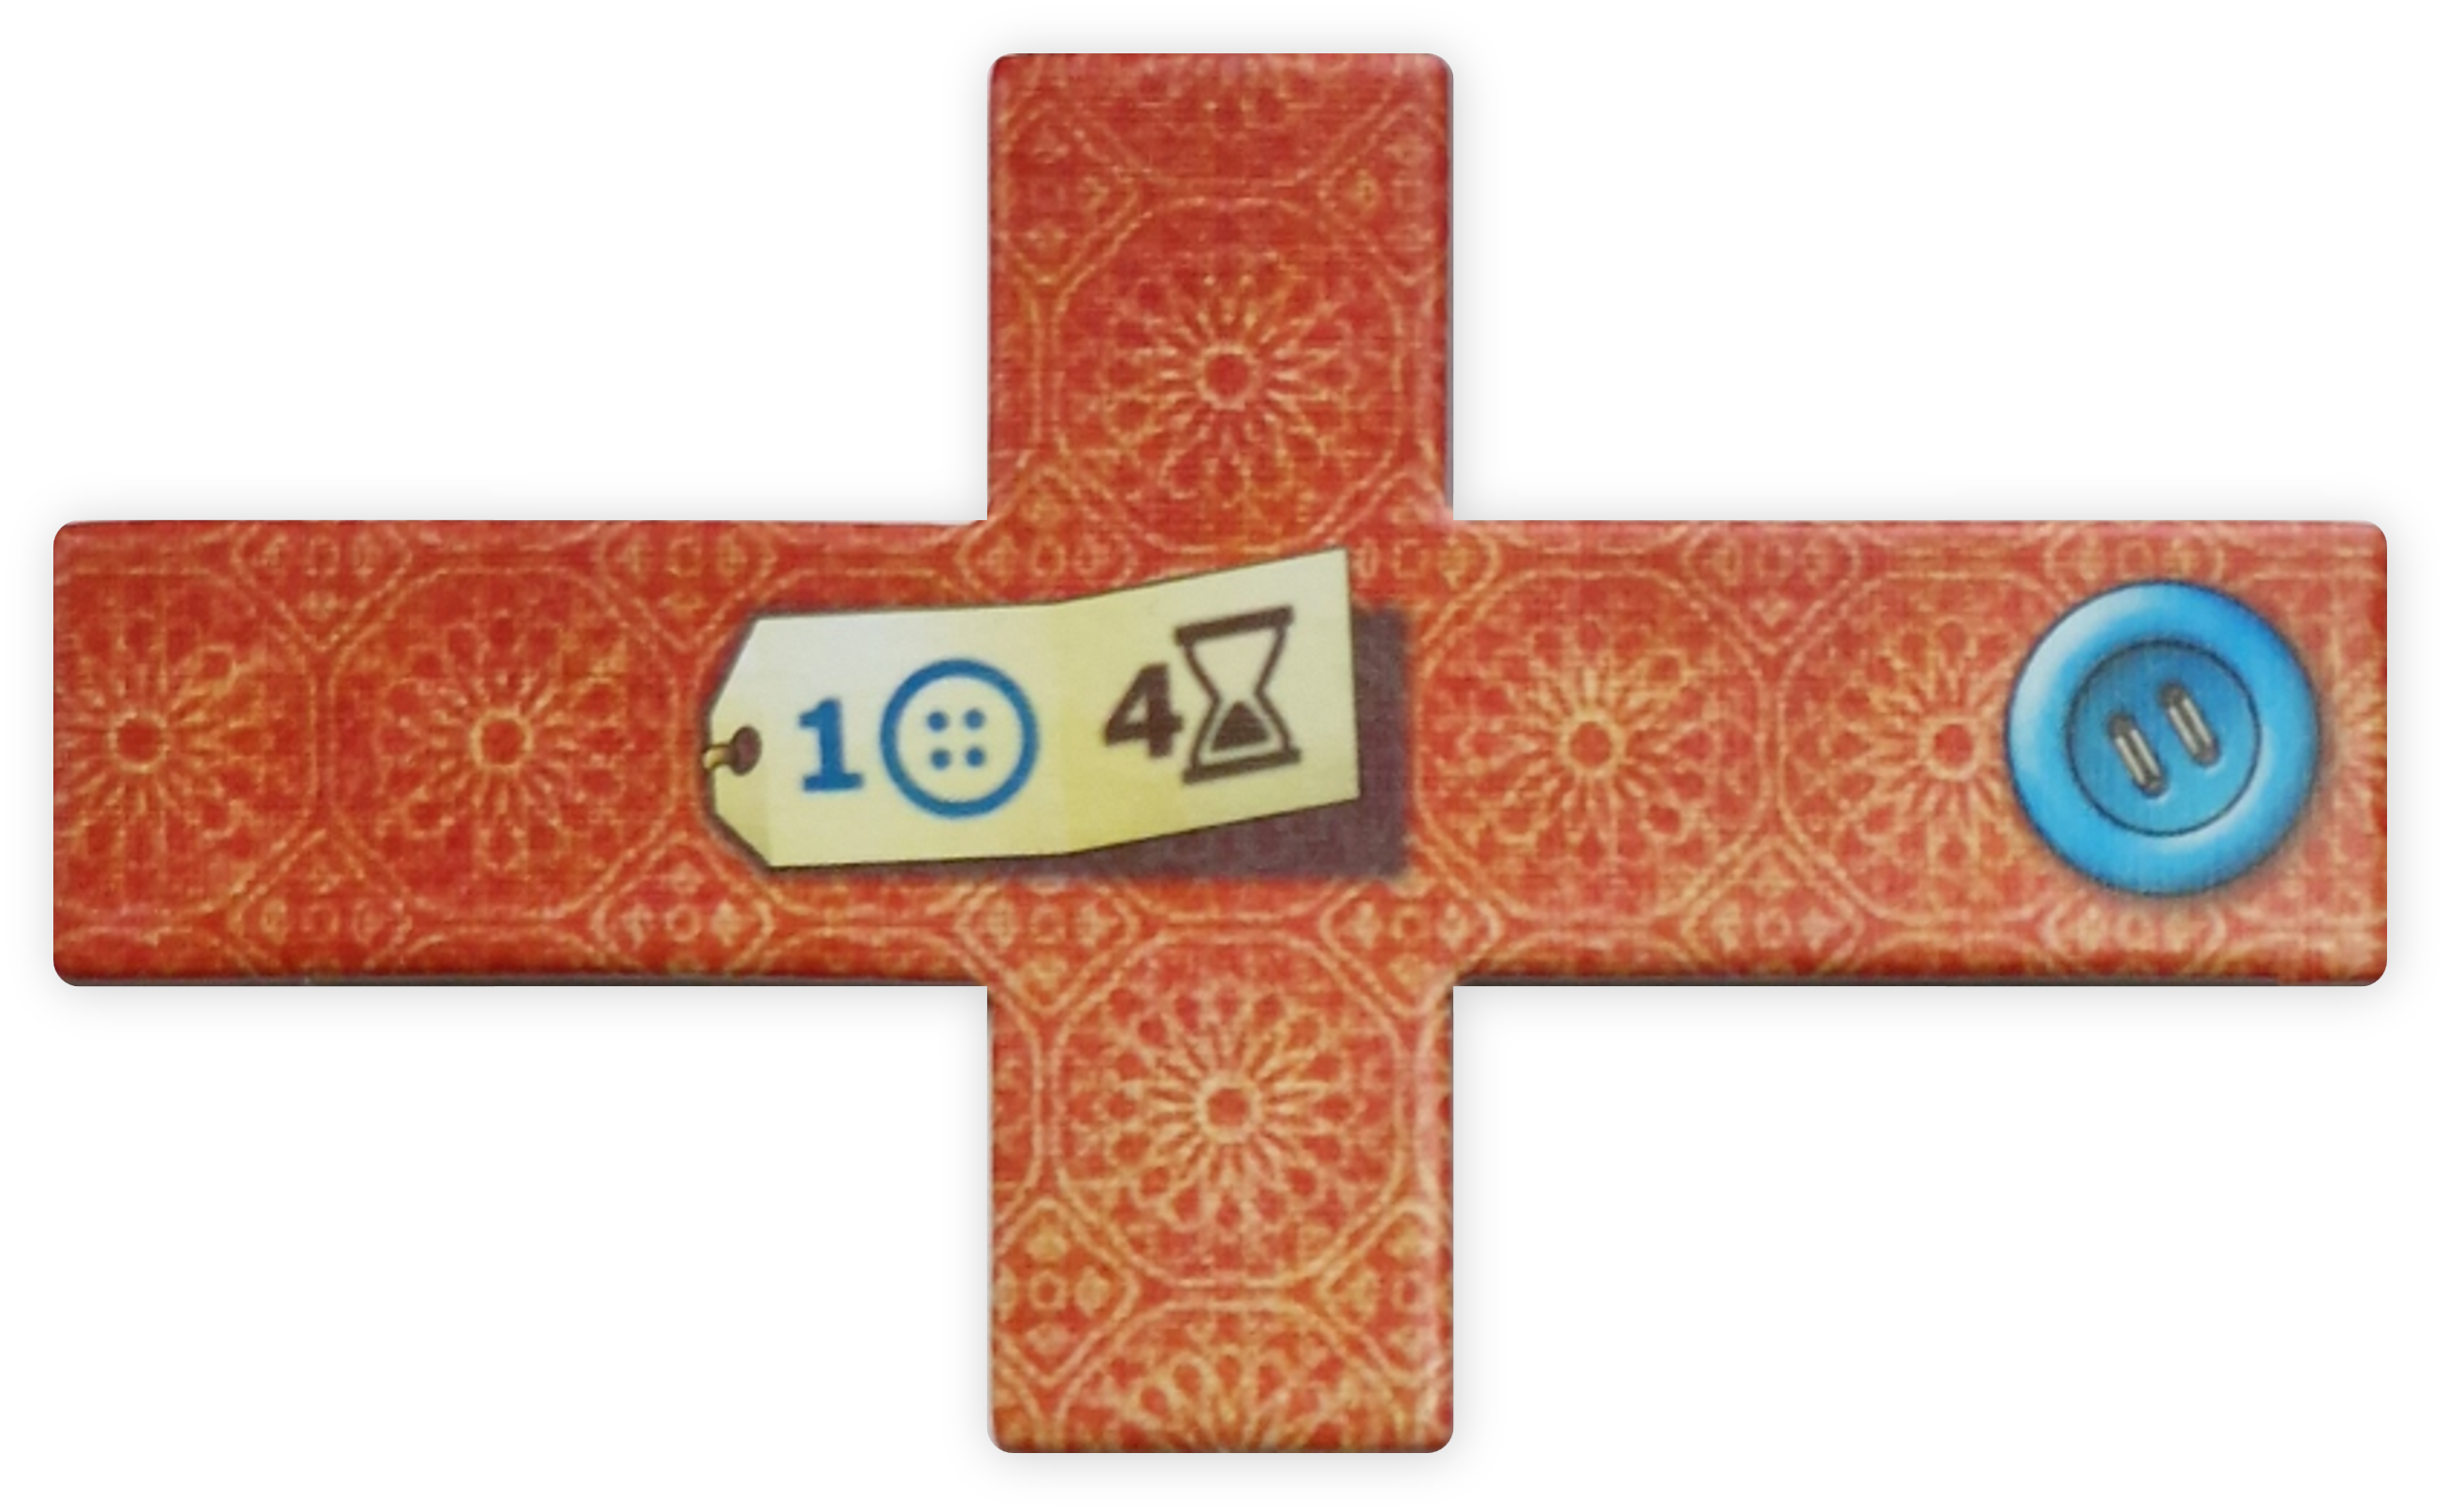
\includegraphics[width=25mm]{res/pictures/assets/20-front.png}};
            \draw[arrow] (walk2c) -- (take20);

            % parallel
            %     c) walk 4, take 11, walk 1, take 6
            \node[left = 2.35cm of take20] (walk4p3) {4 laufen};
            \node[take=11, left = of walk4p3] (take11c) {\includegraphics[width=20mm]{res/pictures/assets/11-front.png}};
            \node[left = of take11c] (walk1p3) {1 laufen};
            \node[take=6, left = of walk1p3] (take06c) {\includegraphics[width=15mm]{res/pictures/assets/06-front.png}};
            \draw[arrow] (take20) -- (walk4p3);
            \draw[arrow] (walk4p3) -- (take11c);
            \draw[arrow] (take11c) -- (walk1p3);
            \draw[arrow] (walk1p3) -- (take06c);
            %     b) walk 4, take 6, walk 1, take 11
            \node[above = 2cm of walk4p3] (walk4p2) {4 laufen};
            \node[take=6, left = of walk4p2] (take06b) {\includegraphics[width=15mm]{res/pictures/assets/06-front.png}};
            \node[left = of take06b] (walk1p2) {1 laufen};
            \node[take=11, left = of walk1p2] (take11b) {\includegraphics[width=20mm]{res/pictures/assets/11-front.png}};
            \draw[arrow] (take20) -|- (walk4p2);
            \draw[arrow] (walk4p2) -- (take06b);
            \draw[arrow] (take06b) -- (walk1p2);
            \draw[arrow] (walk1p2) -- (take11b);
            %     a) walk 4, take 6, take 11, walk 1
            \node[above = 2cm of walk4p2] (walk4p1) {4 laufen};
            \node[take=6, left = of walk4p1] (take06a) {\includegraphics[width=15mm]{res/pictures/assets/06-front.png}};
            \node[take=11, left = of take06a] (take11a) {\includegraphics[width=20mm]{res/pictures/assets/11-front.png}};
            \node[left = of take11a] (walk1p1) {1 laufen};
            \draw[arrow] (take20) -|- (walk4p1);
            \draw[arrow] (walk4p1) -- (take06a);
            \draw[arrow] (take06a) -- (take11a);
            \draw[arrow] (take11a) -- (walk1p1);
            %     d) walk 4, take 11, take 6, walk 1
            \node[below = 1.9cm of walk4p3] (walk4p4) {4 laufen};
            \node[take=11, left = of walk4p4] (take11d) {\includegraphics[width=20mm]{res/pictures/assets/11-front.png}};
            \node[take=6, left = of take11d] (take06d) {\includegraphics[width=15mm]{res/pictures/assets/06-front.png}};
            \node[left = of take06d] (walk1p4) {1 laufen};
            \draw[arrow] (take20) -|- (walk4p4);
            \draw[arrow] (walk4p4) -- (take11d);
            \draw[arrow] (take11d) -- (take06d);
            \draw[arrow] (take06d) -- (walk1p4);
            %     e) ...
            \node (dots) at ($(take11d)!0.5!(take06d) - (0,2)$) {$\dots$};
            \draw[arrow, shorten >=20pt] (take20) -|-[ratio=0.1675] (dots);
            %     f) take 6, walk 5, take 11
            %     g) take 11, walk 5, take 6
            %     h) take 6, take 11, walk 3, walk 2
            %     i) take 11, take 6, walk 3, walk 2

            % take 16
            \node[take=16, left = 2.35cm of take06c] (take16) {\includegraphics[width=10mm]{res/pictures/assets/16-front.png}};
            \draw[arrow] (walk1p1) -|- (take16);
            \draw[arrow] (take11b) -|- (take16);
            \draw[arrow] (take06c) -- (take16);
            \draw[arrow] (walk1p4) -|- (take16);
            \draw[arrow, shorten <=20pt] (dots) -|-[ratio=0.8275] (take16);

            % end
            \node[draw, circle, inner sep=2pt, label=below:Ende] (end) at (start |- take16)  {};
            \draw[arrow] (take16) -- (end);
        \end{tikzpicture}
    \end{adjustbox}
    \vspace*{-0.65cm}
    \caption{Perfektes Patchwork Spiel \textendash{} Alternative 2}
    \label{fig:max-score-turns-alternative-2}
\end{figure}

\vspace*{-1cm}

% OLD: 84 Points Game
% parallel
%     take 17, take 32
%     take 32, take 17
% walk 2
% take 30
% take 4
% take 3
% take 1
% parallel
%     take 6, take 12
%     take 12, take 6
% take 10
% take 26
% take 20
% parallel
%     take 11, walk 1, take 22,
%     walk 1, take 11, take 22,
%     take 22, walk 1, take 11,
%     walk 1, take 22, take 11
% walk 2 (for special patch)
% walk 2
% take 16
% \begin{figure}[!ht]
%     \centering
%     \begin{adjustbox}{width=\textwidth,keepaspectratio}
%         \begin{tikzpicture}[
%             arrow/.style={->, very thick, shorten >=2pt, shorten <=2pt}
%             ]
%
%             \tikzset{
%                 take/.style={inner sep=0,outer sep=0, label=below:#1 nehmen},
%             }
%
%             \node[draw, circle, inner sep=2pt, label=below:Start] (start) at (0,0) {};
%
%             \node[take=32, above right = 1cm and 2cm of start] (take32a) {\includegraphics[width=20mm]{res/pictures/assets/32-front.png}};
%             \node[take=17, right = of take32a] (take17a)  {\includegraphics[width=15mm]{res/pictures/assets/17-front.png}};
%
%             \node[take=17, below right = 1cm and 2cm of start] (take17b)  {\includegraphics[width=15mm]{res/pictures/assets/17-front.png}};
%             \node[take=32, right = of take17b] (take32b) {\includegraphics[width=20mm]{res/pictures/assets/32-front.png}};
%
%             \node[right = 3cm of start -| take17a] (walk2) {2 laufen};
%
%             \node[take=30, right = of walk2] (take30) {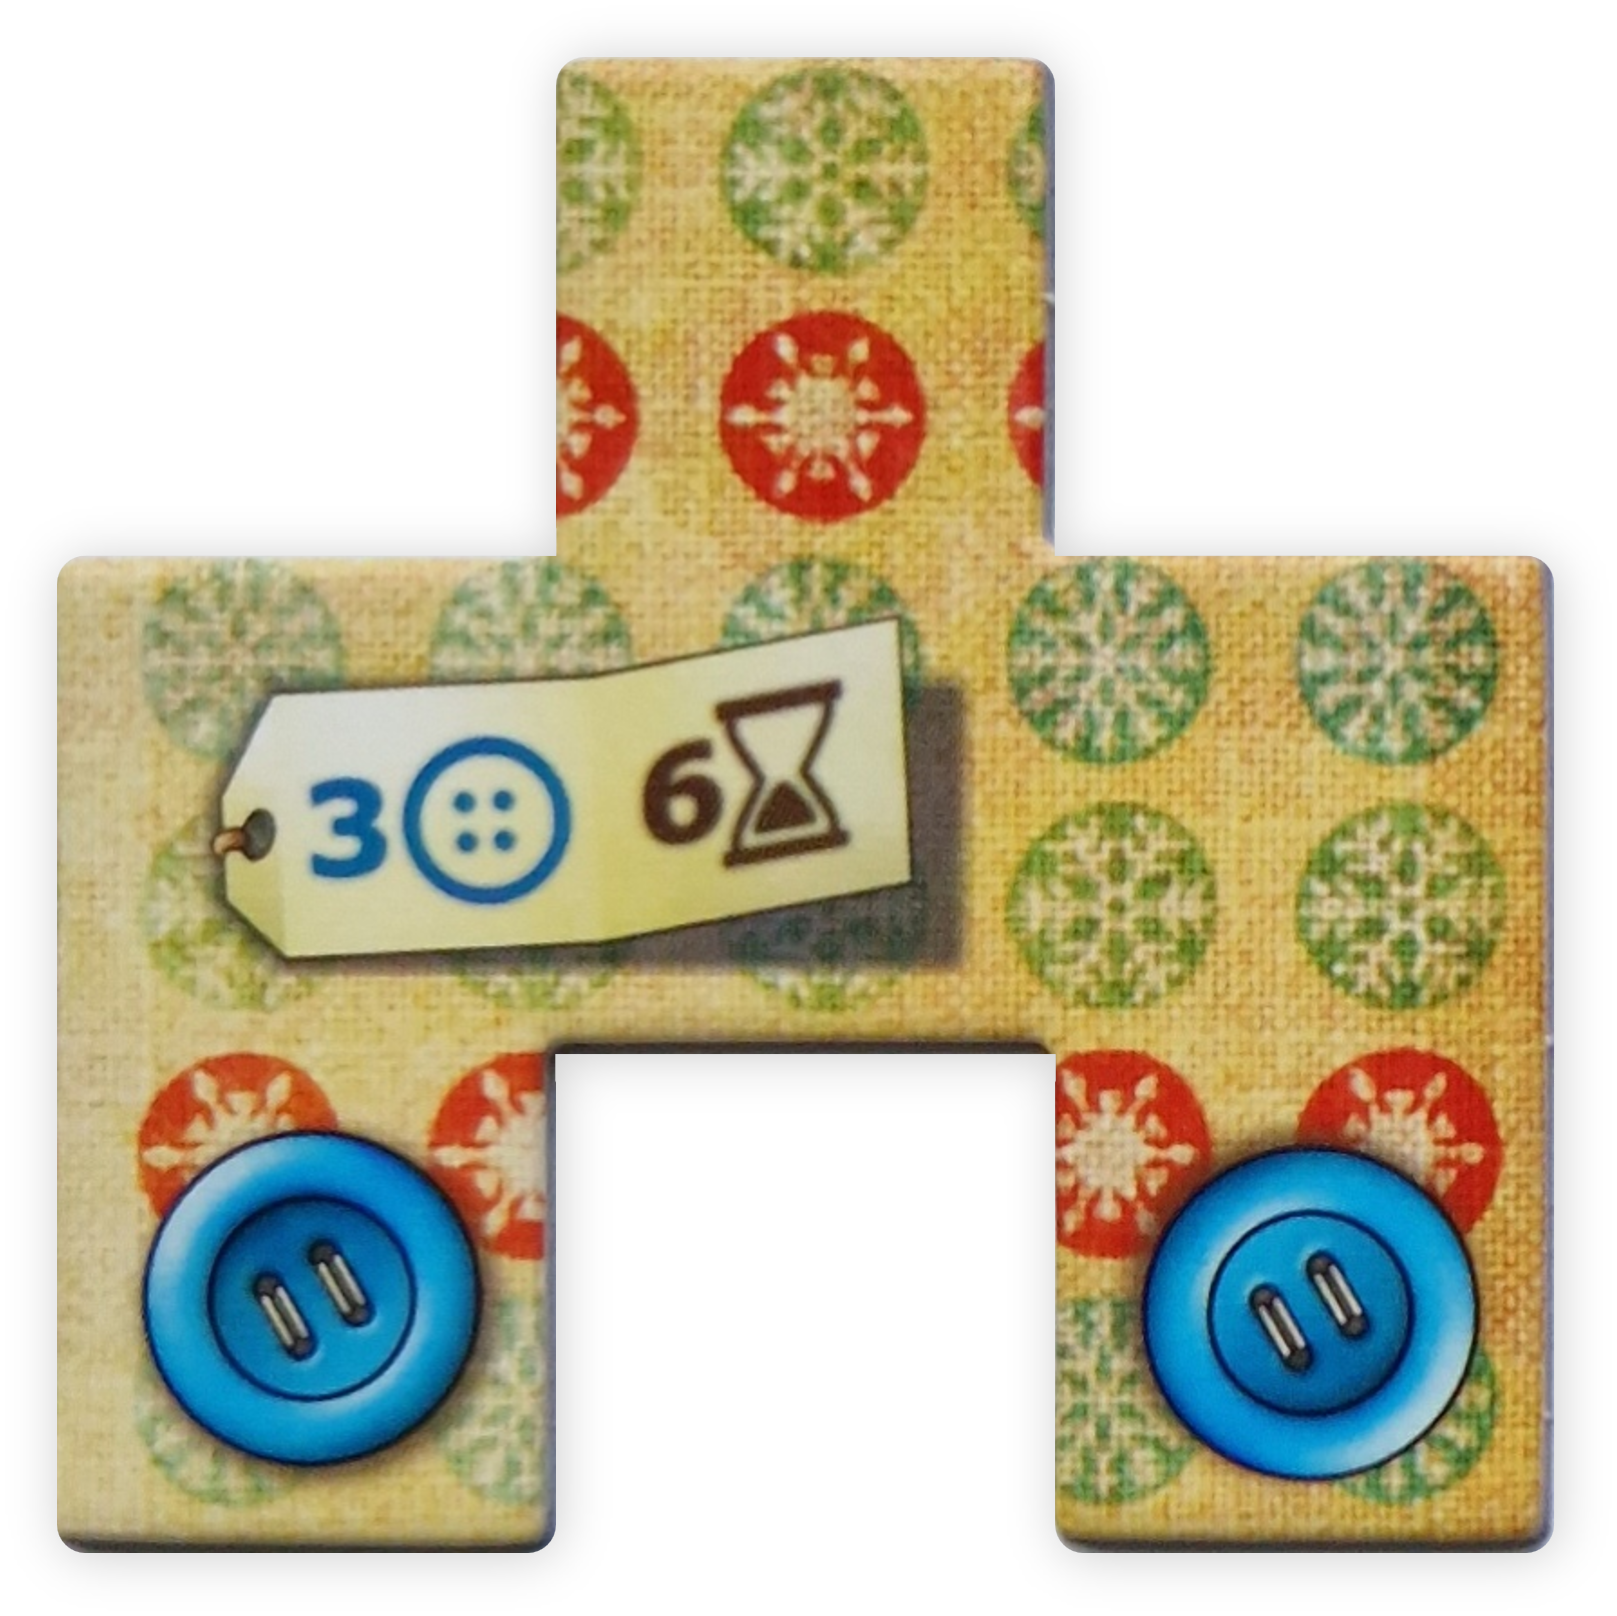
\includegraphics[width=15mm]{res/pictures/assets/30-front.png}};
%             \node[take=4, right = of take30] (take04) {\includegraphics[width=15mm]{res/pictures/assets/04-front.png}};
%             \node[take=3, right = of take04] (take03) {\includegraphics[width=15mm]{res/pictures/assets/03-front.png}};
%             \node[take=1, right = of take03] (take01) {\includegraphics[width=15mm]{res/pictures/assets/01-front.png}};
%
%             \node[take=6, above right = 0cm and 2cm of take01] (take06a) {\includegraphics[width=15mm]{res/pictures/assets/06-front.png}};
%             \node[take=12, right = of take06a] (take12a) {\includegraphics[width=15mm]{res/pictures/assets/12-front.png}};
%
%             \node[take=12, below right = 0cm and 2cm of take01] (take12b) {\includegraphics[width=15mm]{res/pictures/assets/12-front.png}};
%             \node[take=6, right = of take12b] (take06b) {\includegraphics[width=15mm]{res/pictures/assets/06-front.png}};
%
%             \node[take=10, right = 3cm of start -| take12a] (take10) {\includegraphics[width=10mm]{res/pictures/assets/10-front.png}};
%
%             \node[take=26, below = 4cm of take06b -| take10] (take26) {\includegraphics[width=10mm]{res/pictures/assets/26-front.png}};
%             \node[take=20, left = 3cm of take26] (take20) {\includegraphics[width=25mm]{res/pictures/assets/20-front.png}};
%
%             \node[above left = 0.1cm and 4.5cm of take20] (walk1b) {1 laufen};
%             \node[take=11, left = of walk1b] (take11b) {\includegraphics[width=20mm]{res/pictures/assets/11-front.png}};
%             \node[take=22, left = of take11b] (take22b) {\includegraphics[width=15mm]{res/pictures/assets/22-front.png}};
%
%             \node[take=11, above = 1.3cm of walk1b] (take11a) {\includegraphics[width=20mm]{res/pictures/assets/11-front.png}};
%             \node[left = of take11a] (walk1a) {1 laufen};
%             \node[take=22, left = of walk1a] (take22a) {\includegraphics[width=15mm]{res/pictures/assets/22-front.png}};
%
%             \node[take=22, below left = 0.1cm and 4.5cm of take20] (take22c) {\includegraphics[width=15mm]{res/pictures/assets/22-front.png}};
%             \node[left = of take22c] (walk1c) {1 laufen};
%             \node[take=11, left = of walk1c] (take11c) {\includegraphics[width=20mm]{res/pictures/assets/11-front.png}};
%
%             \node[below=1.3cm of take22c] (walk1d) {1 laufen};
%             \node[take=22, left = of walk1d] (take22d) {\includegraphics[width=15mm]{res/pictures/assets/22-front.png}};
%
%             \node[left = 4.5cm of take20 -| take11d] (walk2x2a) {2 laufen};
%             \node[left = of walk2x2a] (walk2x2b) {2 laufen};
%
%             \node[take=16, left = of walk2x2b] (take16) {\includegraphics[width=10mm]{res/pictures/assets/16-front.png}};
%
%             \node[draw, circle, inner sep=2pt, label=below:Ende] (end) at (start |- take16)  {};
%
%             \draw[arrow] (start) -|- (take32a);
%             \draw[arrow] (start) -|- (take17b);
%             \draw[arrow] (take32a) -- (take17a);
%             \draw[arrow] (take17b) -- (take32b);
%             \draw[arrow] (take17a) -|- (walk2);
%             \draw[arrow] (take32b) -|- (walk2);
%             \draw[arrow] (walk2) -- (take30);
%             \draw[arrow] (take30) -- (take04);
%             \draw[arrow] (take04) -- (take03);
%             \node[take=11, left = of take22d] (take11d) {\includegraphics[width=20mm]{res/pictures/assets/11-front.png}};
%             \draw[arrow] (take03) -- (take01);
%             \draw[arrow] (take01) -|- (take06a);
%             \draw[arrow, shorten <=20pt] (take01) -|- (take12b);
%             \draw[arrow] (take06a) -- (take12a);
%             \draw[arrow] (take12b) -- (take06b);
%             \draw[arrow] (take12a) -|- (take10);
%             \draw[arrow] (take06b) -|- (take10);
%             \draw[arrow, shorten <=20pt] (take10) -- (take26);
%             \draw[arrow] (take26) -- (take20);
%
%             \draw[arrow] (take20) -|-[ratio=.672] (take11a);
%             \draw[arrow] (take20) -|-[ratio=.65] (walk1b);
%             \draw[arrow] (take20) -|-[ratio=.65] (take22c);
%             \draw[arrow] (take20) -|-[ratio=.6605] (walk1d);
%
%             \draw[arrow] (take11a) -- (walk1a);
%             \draw[arrow] (walk1a) -- (take22a);
%             \draw[arrow] (walk1b) -- (take11b);
%             \draw[arrow] (take11b) -- (take22b);
%             \draw[arrow] (take22c) -- (walk1c);
%             \draw[arrow] (walk1c) -- (take11c);
%             \draw[arrow] (walk1d) -- (take22d);
%             \draw[arrow] (take22d) -- (take11d);
%
%             \draw[arrow] (take22a) -|-[ratio=.52] (walk2x2a);
%             \draw[arrow] (take22b) -|-[ratio=.5] (walk2x2a);
%             \draw[arrow] (take11c) -|-[ratio=.5] (walk2x2a);
%             \draw[arrow] (take11d) -|-[ratio=.51] (walk2x2a);
%
%             \draw[arrow] (walk2x2a) -- (walk2x2b);
%             \draw[arrow] (walk2x2b) -- (take16);
%             \draw[arrow] (take16) -- (end);
%
%         \end{tikzpicture}
%     \end{adjustbox}
%     % \vspace*{-0.5cm}
%     \caption{Perfektes Patchwork Spiel}
%     \label{fig:max-score-turns-old}
% \end{figure}

\pagebreak

\section{Ablagepläne}
\label{anhang:section-ablageplaene}

\subsection{Ablageplan für perfektes Patchwork Spiel \textendash{} Alternative 1}
\label{anhang:section-ablageplan-perfektes-spiel-alternative-1}

\begin{figure}[!ht]
    \centering
    \begin{tikzpicture}
        \node [inner sep=0pt,outer sep=0pt,clip,rounded corners=0.15cm] (image) at (0,0) {\includegraphics[width=0.375\textwidth]{res/pictures/perfect-game.jpg}};
        \drawshadow{image}
    \end{tikzpicture}
    \caption{Ablageplan beim perfekten Spiel \textendash{} Alternative 1}
    \label{fig:max-score-quilt-board-alternative-1}
\end{figure}

\subsection{Ablageplan für perfektes Patchwork Spiel \textendash{} Alternative 2}
\label{anhang:section-ablageplan-perfektes-spiel-alternative-2}

\begin{figure}[!ht]
    \centering
    \begin{tikzpicture}
        \node [inner sep=0pt,outer sep=0pt,clip,rounded corners=0.15cm] (image) at (0,0) {\includegraphics[width=0.375\textwidth]{res/pictures/perfect-game-alternative.jpg}};
        \drawshadow{image}
    \end{tikzpicture}
    \caption{Ablageplan beim perfekten Spiel \textendash{} Alternative 2}
    \label{fig:max-score-quilt-board-alternative-2}
\end{figure}
